\section{Queuing Model (90 pts)\label{sec:7}}

    The last section concentrates on theoretical foundations and we apply different modelling techniques and observe how
    the real system's results differ from computed ones. Explanations for discrepancies and overlaps between computer
    values and measured results are given.

    This section includes the M/M/1 and M/M/m model (which use data from experiment \ref{sec:4} as the basis) as well as a
    network of queues which tries to attain results for configurations of experiment \ref{sec:3}.

    For M/M/1 and M/M/m models the following parameters are part of the system.

    Input Parameters:
    \begin{itemize}
        \item $\mu$: The service rate of the system. It is calculated from the maximally observed average throughput
              from any single run for a given amount of worker threads in experiment \ref{sec:4} disregarding the
              response time reported. This number is divided by twice the number of worker threads for M/M/m models. The
              actual value used is documented in the respective table.
        \item $\lambda$: The arrival rate of jobs. It is taken directly from observed results of the average throughput
              for both middlewares for all repetitions of an experiment. This number is included in the table as well.
        \item $m$: The number of services. It is only relevant for the M/M/m models. The service count is double the
              amount of worker threads configured as two \mw{}s are used.
    \end{itemize}

    Output Parameters:
    \begin{itemize}
        \item $\rho$: The traffic intensity. For the M/M/m model this is equivalent to $U$, the average utilization of
              each server.
        \item $\mathbb{E}[n]$: Expected number of jobs in the system.
        \item $\mathbb{E}[n_q]$: Expected number of jobs in the queue.
        \item $\mathbb{E}[w]$: Expected waiting time for elements in the queue.
        \item $\mathbb{E}[r]$: Expected response time of the system.
        \item $p_0$: Probability of zero jobs in the system. Only relevant for the M/M/m model.
        \item $\varrho$: Probability of queueing. Only relevant for the M/M/m model.
    \end{itemize}

    Choosing the service rate and arrival rate as described gives for all following calculations the guarantee that
    $\rho < 1$ holds as the averaged throughput for all repetitions is expected to be smaller than any maximally
    observed value. This is a stability parameter which needs to hold for calculations to be valid as the system would
    otherwise not be fulfilling the requirements of an M/M/1 or M/M/m model.

    \subsection{M/M/1\label{subsec:7_mm1}}
        The M/M/1 model is a simple model which is founded the idea of only containing a single queue and service. Jobs to
        this system arrive with a mean arrival rate of $\lambda$ and are processed by the service with the mean service
        rate $\mu$.

        In table \ref{tab:mm1} the computed results for all combinations of worker threads with clients are presented
        for the M/M/m model. Comparing the received numbers with measured data it becomes clear this model is
        insufficient to describe the real system's behaviour.

        The following observations are made:

        \begin{enumerate}
            \item The trend to a decreased response time for more worker threads is valid the M/M/1 model and the real
                  system. The response time compared to is the true response time of the middleware for a memtier
                  request.
            \item The queue times are estimated too close to the estimated response times and are in many cases a couple
                  hundred microseconds quicker. This is not valid in the real model as network communication is not
                  modelled. The real system must not only process the packet it must also distribute the SET requests to
                  each \srv{} connected, wait for replies and then send back the response to memtier. This is simply not
                  modelled by M/M/1.
            \item The queue sizes show also a trend towards smaller sizes for more clients with larger worker threads.
                  Queues are mostly modelled too large compared with the real system and therefore overestimate the
                  amount of queueing. This is expected as a single queue is used by the model. As such the observation
                  of the number of elements in the system being larger by at most one element compared to the number of
                  queues can be explained.\newline
                  The trend is only a trend and not the true cause for the over-estimation. The queue size is only
                  determined by $\rho$ and as such actually independent of the number of clients and worker threads.
        \end{enumerate}

        Overall the model is at most a vague approximation as it is a sequential, single queue and single service model
        whereas the middleware is a model of multiple concurrent services with two queues.

        \begin{table}
            \footnotesize{
                \begin{tabular}{lllrrrrrrrrrrrr}
                    \toprule
                    & & & & & \multicolumn{2}{c}{$\mathbb{E}[n_q]$} & \multicolumn{2}{c}{$\mathbb{E}[w]$} & \multicolumn{2}{c}{$\mathbb{E}[r]$} & \\
                    \cmidrule(lr){6-7}
                    \cmidrule(lr){8-9}
                    \cmidrule(lr){10-11}
                    Clients & WT & $\mu$        & $\lambda$ & $\rho$ & Act.   & Est.   & Act.  & Est.  & Act.  & Est.  & $\mathbb{E}[n]$ \\
                    \midrule
                    6       & 8  & 6750.87  & 2840.72   & 0.42   & 0.55   & 0.31   & 0.06  & 0.11  & 1.31  & 0.26  & 0.73    \\
                            & 16 & 8716.58  & 2841.52   & 0.33   & 0.55   & 0.16   & 0.06  & 0.06  & 1.32  & 0.17  & 0.48    \\
                            & 32 & 10385.53 & 2804.02   & 0.27   & 0.55   & 0.10   & 0.06  & 0.04  & 1.35  & 0.13  & 0.37    \\
                            & 64 & 11582.18 & 2795.48   & 0.24   & 0.54   & 0.08   & 0.07  & 0.03  & 1.38  & 0.11  & 0.32    \\
                    \addlinespace
                    12      & 8  & 6750.87  & 4967.16   & 0.74   & 0.71   & 2.05   & 0.08  & 0.41  & 1.62  & 0.56  & 2.78    \\
                            & 16 & 8716.58  & 4912.71   & 0.56   & 0.71   & 0.73   & 0.08  & 0.15  & 1.64  & 0.26  & 1.29    \\
                            & 32 & 10385.53 & 4916.28   & 0.47   & 0.70   & 0.43   & 0.08  & 0.09  & 1.64  & 0.18  & 0.90    \\
                            & 64 & 11582.18 & 4837.95   & 0.42   & 0.71   & 0.30   & 0.09  & 0.06  & 1.69  & 0.15  & 0.72    \\
                    \addlinespace
                    24      & 8  & 6750.87  & 5955.70   & 0.88   & 1.34   & 6.61   & 0.71  & 1.11  & 3.13  & 1.26  & 7.49    \\
                            & 16 & 8716.58  & 6152.89   & 0.71   & 1.27   & 1.69   & 0.16  & 0.28  & 3.00  & 0.39  & 2.40    \\
                            & 32 & 10385.53 & 6152.39   & 0.59   & 1.24   & 0.86   & 0.15  & 0.14  & 3.02  & 0.24  & 1.45    \\
                            & 64 & 11582.18 & 6065.53   & 0.52   & 1.27   & 0.58   & 0.15  & 0.09  & 3.06  & 0.18  & 1.10    \\
                    \addlinespace
                    48      & 8  & 6750.87  & 6680.05   & 0.99   & 10.97  & 93.34  & 3.82  & 13.97 & 6.26  & 14.12 & 94.33   \\
                            & 16 & 8716.58  & 8187.89   & 0.94   & 2.90   & 14.55  & 1.17  & 1.78  & 4.82  & 1.89  & 15.49   \\
                            & 32 & 10385.53 & 8378.57   & 0.81   & 2.52   & 3.37   & 0.30  & 0.40  & 4.66  & 0.50  & 4.17    \\
                            & 64 & 11582.18 & 8169.04   & 0.71   & 2.54   & 1.69   & 0.32  & 0.21  & 4.78  & 0.29  & 2.39    \\
                    \addlinespace
                    96      & 8  & 6750.87  & 6664.46   & 0.99   & 34.90  & 76.14  & 11.03 & 11.43 & 13.47 & 11.57 & 77.13   \\
                            & 16 & 8716.58  & 8615.87   & 0.99   & 23.51  & 84.56  & 6.28  & 9.81  & 10.05 & 9.93  & 85.55   \\
                            & 32 & 10385.53 & 10010.31  & 0.96   & 6.97   & 25.71  & 2.04  & 2.57  & 8.11  & 2.67  & 26.68   \\
                            & 64 & 11582.18 & 9934.78   & 0.86   & 5.23   & 5.17   & 0.72  & 0.52  & 7.88  & 0.61  & 6.03    \\
                    \addlinespace
                    192     & 8  & 6750.87  & 6690.19   & 0.99   & 82.90  & 109.27 & 25.35 & 16.33 & 27.79 & 16.48 & 110.26  \\
                            & 16 & 8716.58  & 8626.23   & 0.99   & 71.39  & 94.49  & 17.41 & 10.95 & 21.17 & 11.07 & 95.48   \\
                            & 32 & 10385.53 & 10327.67  & 0.99   & 50.35  & 177.48 & 10.70 & 17.18 & 16.95 & 17.28 & 178.47  \\
                            & 64 & 11582.18 & 11250.96  & 0.97   & 16.84  & 33.00  & 3.51  & 2.93  & 14.20 & 3.02  & 33.97   \\
                    \addlinespace
                    288     & 8  & 6750.87  & 6721.16   & 1.00   & 130.85 & 225.26 & 39.52 & 33.52 & 41.95 & 33.66 & 226.26  \\
                            & 16 & 8716.58  & 8681.76   & 1.00   & 119.31 & 248.28 & 28.35 & 28.60 & 32.09 & 28.71 & 249.28  \\
                            & 32 & 10385.53 & 10366.34  & 1.00   & 98.10  & 539.23 & 19.94 & 52.02 & 26.17 & 52.11 & 540.23  \\
                            & 64 & 11582.18 & 11468.23  & 0.99   & 56.99  & 99.65  & 10.73 & 8.69  & 21.87 & 8.78  & 100.64  \\
                    \bottomrule
                \end{tabular}
                \caption{M/M/1 calculations for given configurations of Experiment 4 using the formulae listed in
                         the book, Box 31.1. Numbers are rounded to two decimal places for presentation
                         purposes which for the case of $\rho$ makes the system seem unstable yet the actual numbers are
                         $< 1$.\label{tab:mm1}}
            }
        \end{table}

    \subsection{M/M/m\label{subsec:7_mmm}}
        The M/M/m model is an extension to the M/M/1 model which still keeps the single queue but has $m$ services. These
        services will be modelled by the amount of total worker threads in the system. With 2 \mw{}s $m$ is set to
        double the value of worker threads (and not explicitly documented in the table).

        In table \ref{tab:mmm} the computed results for all combinations of worker threads with clients are presented
        for the M/M/m model. Comparing the received numbers with measured data it becomes clear this model is still
        insufficient to describe the real system's behaviour.

        The following observations are made:

        \begin{enumerate}
            \item The trend to decreased response times is not holding, response times are actually growing for
                  increasing amounts of worker threads. This stems from the choice of $\mu$ not increasing but
                  decreasing when increasing worker threads as the average request throughput per service is decreasing
                  due to scheduling overhead in the real system.
            \item The queue times are not in the vicinity of a couple hundred microseconds anymore when compared to the
                  response time but reflect more the actual observed difference between observed response time and
                  observed queue time. Overall the queue waiting times are not in general matching the system.
            \item The queue sizes still show a towards smaller sizes for more clients with larger worker threads. For
                  the M/M/m calculaton there is also the inclusion of the parameter $\varrho$ in the number of elements in
                  the queue. With he factor approaching 1 with high loads it is expected that the M/M/m model shows
                  similar behaviour to the M/M/1 model. For the queue size this can be observed by comparing results from
                  tables \ref{tab:7_mm1} and \ref{tab:7_mmm}. For low workloads smaller queue sizes are predicted. With
                  such a system which is quite binary few predictions matching the real system are expected.
            \item The probability of queueing goes up for more load (which is expected). The probability seem low
                  compared to the actually observed queue-sizes for experiment \ref{sec:4}, meaning queuing expectations
                  should be converging earlier to 1.
            \item The probability of 0 jobs in the system is 0 for all experiments. This matches the expected reality.
            \item The elements in the system don't correlate anymore directly with the queuesize. The numbers are in the
                  case of low workloads not matching the expectation and suggest jobs to exist for client counts which
                  shouldn't allow such high numbers,
        \end{enumerate}

        Overall the model is better but not by much as it may be parallel but still it uses a single queue. The
        middleware does use multiple concurrent services but uses two, instead of one queue. Additionally this system
        merges the worker threads and memcached into one virtual service, clearly not the actual system behaviour.

        \begin{table}
            \begin{adjustwidth}{-1cm}{}
                \footnotesize{
                    \begin{tabular}{lllrrrrrrrrrrrr}
                        \toprule
                        & & & & & \multicolumn{2}{c}{$\mathbb{E}[n_q]$} & \multicolumn{2}{c}{$\mathbb{E}[w]$} & \multicolumn{2}{c}{$\mathbb{E}[r]$} & &  & & \\
                        \cmidrule(lr){6-7}
                        \cmidrule(lr){8-9}
                        \cmidrule(lr){10-11}
                        Clients & WT & $\mu$      & $\lambda$ & $\rho$ & Act.   & Est.   & Act.  & Est.  & Act.  & Est.  & $\mathbb{E}[n]$ & $\varrho$ & $p_0$ & $U$ \\
                        \midrule
                        6       & 8  & 421.93 & 2840.72   & 0.42   & 0.55   & 0.00   & 0.06  & 0.00  & 1.31  & 2.37  & 6.73            & 0.00      & 0.0   & 0.42 \\
                                & 16 & 272.39 & 2841.52   & 0.33   & 0.55   & 0.00   & 0.06  & 0.00  & 1.32  & 3.67  & 10.43           & 0.00      & 0.0   & 0.33 \\
                                & 32 & 162.27 & 2804.02   & 0.27   & 0.55   & 0.00   & 0.06  & 0.00  & 1.35  & 6.16  & 17.28           & 0.00      & 0.0   & 0.27 \\
                                & 64 & 90.49  & 2795.48   & 0.24   & 0.54   & 0.00   & 0.07  & 0.00  & 1.38  & 11.05 & 30.89           & 0.00      & 0.0   & 0.24 \\
                        \addlinespace
                        12      & 8  & 421.93 & 4967.16   & 0.74   & 0.71   & 0.50   & 0.08  & 0.10  & 1.62  & 2.47  & 12.28           & 0.18      & 0.0   & 0.74 \\
                                & 16 & 272.39 & 4912.71   & 0.56   & 0.71   & 0.00   & 0.08  & 0.00  & 1.64  & 3.67  & 18.04           & 0.00      & 0.0   & 0.56 \\
                                & 32 & 162.27 & 4916.28   & 0.47   & 0.70   & 0.00   & 0.08  & 0.00  & 1.64  & 6.16  & 30.30           & 0.00      & 0.0   & 0.47 \\
                                & 64 & 90.49  & 4837.95   & 0.42   & 0.71   & 0.00   & 0.09  & 0.00  & 1.69  & 11.05 & 53.47           & 0.00      & 0.0   & 0.42 \\
                        \addlinespace
                        24      & 8  & 421.93 & 5955.70   & 0.88   & 1.34   & 3.98   & 0.71  & 0.67  & 3.13  & 3.04  & 18.10           & 0.53      & 0.0   & 0.88 \\
                                & 16 & 272.39 & 6152.89   & 0.71   & 1.27   & 0.10   & 0.16  & 0.02  & 3.00  & 3.69  & 22.69           & 0.04      & 0.0   & 0.71 \\
                                & 32 & 162.27 & 6152.39   & 0.59   & 1.24   & 0.00   & 0.15  & 0.00  & 3.02  & 6.16  & 37.91           & 0.00      & 0.0   & 0.59 \\
                                & 64 & 90.49  & 6065.53   & 0.52   & 1.27   & 0.00   & 0.15  & 0.00  & 3.06  & 11.05 & 67.03           & 0.00      & 0.0   & 0.52 \\
                        \addlinespace
                        48      & 8  & 421.93 & 6680.05   & 0.99   & 10.97  & 89.74  & 3.82  & 13.43 & 6.26  & 15.80 & 105.57          & 0.95      & 0.0   & 0.99 \\
                                & 16 & 272.39 & 8187.89   & 0.94   & 2.90   & 9.91   & 1.17  & 1.21  & 4.82  & 4.88  & 39.97           & 0.64      & 0.0   & 0.94 \\
                                & 32 & 162.27 & 8378.57   & 0.81   & 2.52   & 0.27   & 0.30  & 0.03  & 4.66  & 6.19  & 51.90           & 0.06      & 0.0   & 0.81 \\
                                & 64 & 90.49  & 8169.04   & 0.71   & 2.54   & 0.00   & 0.32  & 0.00  & 4.78  & 11.05 & 90.28           & 0.00      & 0.0   & 0.71 \\
                        \addlinespace
                        96      & 8  & 421.93 & 6664.46   & 0.99   & 34.90  & 72.56  & 11.03 & 10.89 & 13.47 & 13.26 & 88.36           & 0.94      & 0.0   & 0.99 \\
                                & 16 & 272.39 & 8615.87   & 0.99   & 23.51  & 79.01  & 6.28  & 9.17  & 10.05 & 12.84 & 110.64          & 0.92      & 0.0   & 0.99 \\
                                & 32 & 162.27 & 10010.31  & 0.96   & 6.97   & 18.35  & 2.04  & 1.83  & 8.11  & 8.00  & 80.04           & 0.69      & 0.0   & 0.96 \\
                                & 64 & 90.49  & 9934.78   & 0.86   & 5.23   & 0.35   & 0.72  & 0.04  & 7.88  & 11.09 & 110.15          & 0.06      & 0.0   & 0.86 \\
                        \addlinespace
                        192     & 8  & 421.93 & 6690.19   & 0.99   & 82.90  & 105.65 & 25.35 & 15.79 & 27.79 & 18.16 & 121.51          & 0.96      & 0.0   & 0.99 \\
                                & 16 & 272.39 & 8626.23   & 0.99   & 71.39  & 88.91  & 17.41 & 10.31 & 21.17 & 13.98 & 120.58          & 0.93      & 0.0   & 0.99 \\
                                & 32 & 162.27 & 10327.67  & 0.99   & 50.35  & 168.99 & 10.70 & 16.36 & 16.95 & 22.53 & 232.63          & 0.95      & 0.0   & 0.99 \\
                                & 64 & 90.49  & 11250.96  & 0.97   & 16.84  & 22.23  & 3.51  & 1.98  & 14.20 & 13.03 & 146.57          & 0.65      & 0.0   & 0.97 \\
                        \addlinespace
                        288     & 8  & 421.93 & 6721.16   & 1.00   & 130.85 & 221.60 & 39.52 & 32.97 & 41.95 & 35.34 & 237.53          & 0.98      & 0.0   & 1.00 \\
                                & 16 & 272.39 & 8681.76   & 1.00   & 119.31 & 242.59 & 28.35 & 27.94 & 32.09 & 31.61 & 274.46          & 0.97      & 0.0   & 1.00 \\
                                & 32 & 162.27 & 10366.34  & 1.00   & 98.10  & 530.59 & 19.94 & 51.18 & 26.17 & 57.35 & 594.48          & 0.98      & 0.0   & 1.00 \\
                                & 64 & 90.49  & 11468.23  & 0.99   & 56.99  & 87.54  & 10.73 & 7.63  & 21.87 & 18.68 & 214.28          & 0.87      & 0.0   & 0.99 \\
                        \bottomrule
                    \end{tabular}
                    \caption{M/M/m calculations for given configurations of Experiment 4 using the formulae listed in
                             the book, Box 31.2. Numbers are rounded to two decimal places for presentation purposes
                             which for the case of $\rho$ makes the system seem unstable yet the actual numbers are
                             $< 1$.\label{tab:mmm}}
                }
            \end{adjustwidth}
        \end{table}

        \subsection{Network of Queues\label{subsec:7_noc}}

            In the following two network of queue designs are constructed to try and model results obtained on
            experiments \ref{subsec:3_one-middleware} and \ref{subsec:3_two-middlewares}. The designs include 3 queues
            and 2 latency centers (which emulate the network where applicable).

            A visualization of the network of queues for 2 \mw{}s can be seen in figure \ref{fig:noq_2mw} with the
            difference to model 1 being the existence of only 1 \mw{} instead of two for placement of components. With
            two \mw{}s the requests are split up between both in an even fashion such that both middlewares experience
            only half the throughput.\newline
            As can be seen memcached is modelled with a queue, more specifically using an M/M/1 approach as this reflects
            the experimental setup. Instances of memtier are assumed to be queue-less and their performance being
            infinite. This matches with experimental setups where memtier was not the cause for slowdown (cf. experiment
            \ref{sec:2}). The middleware is modelled with 2 queues, once an M/M/1 queue which emulates the single network
            thread and an M/M/m queue which simulate the workers. The approach to model the network thread with an M/M/1
            queue follows from real system behaviour where packets queue up on a network card if they are not processed
            quick enough. The M/M/m queue for the workers follows from the fact that a single queue is used amongst
            workers from which they take work elements. The decision to leave out modelling the reply stems from the
            fact that the correct pathway would involve the path back from memcached to each worker thread that
            communicated with it and then have it reply back to memtier. With the design not allowing bidirectional
            flows through service centers this cannot be correctly modelled.

            \begin{figure}
                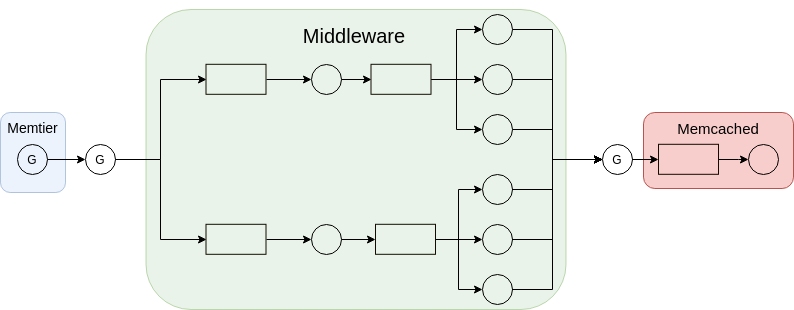
\includegraphics[width=0.7\linewidth]{graphics/network-of-queues_2-middlewares.png}
                \caption{Design of the network of queues. All rectangles define queues, circles delay centers. Circles
                         with a ``G'' define delay centers which allow utilizations above 1 as they model the
                         network.\label{fig:noq_2mw}}
            \end{figure}

            The software package \tw{queueing} from \emph{GNU Octave} is used to model the previously designed networks
            using Mean-Value Analysis. The parameters for both networks are defined as follows:
            \begin{itemize}
                \item $n$: The number of requests in the system. This is equal to the amount of currently active
                      clients.
                \item $S$: The average service time per actor. The actors are defined as follows for the network of
                      queues:
                      \begin{itemize}
                          \item $S_{client}$: It is set to 0 as we assume \cli{}s to never be the bottleneck.
                          \item $S_{network}$: The latency of the network. As a general idea the results from ping are
                                taken and halved. These have been observed in the experiments.
                          \item $S_{netthread}$: The service time of the network thread. This is inferred from the
                                maximum throughput observed in SET requests for the configurations of one and two
                                \mw{}s. For the latter case this number is also halved as two instances exist and on
                                average either has only experienced half the workload.
                          \item $S_{worker}$: The service time per worker. It is inferred for each worker thread and
                                client load configuration separately to model the actual system behaviour in regards to
                                scheduling under more load and clients reasonably. It is derived by taking the response
                                time of the whole system and subtracting the queuing time and memcached communication
                                time.
                          \item $S_{server}$: The service time for memcached. This is inferred from the maximum
                                throughput per request type as GETs are network bound whereas SETs are CPU bound. For
                                all analysis with SET this is $\tfrac{1}{16335}$ (from experiment
                                \ref{subsec:2_one-server}) and for all analysis with GET this is $\tfrac{1}{2940}$ (from
                                experiment \ref{subsec:3_one-middleware} as the throughput is higher compared to
                                experiment \ref{subsec:2_one-server}).
                      \end{itemize}
                \item $V$: The visit ratios from one service center to the next. It is in general set to 1 but for 2
                      \mw{}s the ratio between the network delay center and each M/M/1 queue is halved to model the
                      experimental parameters correctly.
                \item $m$: The number of identical servers for each node. This is only relevant for the M/M/m queues which
                      model multiple concurrent worker threads.
            \end{itemize}

            We observe the results of the MVA in terms of throughput ($X$), response times ($R$), queue sizes ($Q$) and
            system utilization ($U$).

            \begin{table}
                \footnotesize{%
                    \begin{tabular}{llllrrrrrr}
                        \toprule
                        & & & & & & \multicolumn{2}{c}{Worker Threads} & \multicolumn{2}{c}{Memcached} \\
                        \cmidrule(lr){7-8}
                        \cmidrule(lr){9-10}
                        \# MWs & Type & Parameter & $m$ & Delay Center & Net-Thread & Act. & MVA & Act. & MVA \\
                        \midrule
                        1 & GET  & $U$ & 6   & 0.69 & 0.20   & \textemdash & 0.04 & \textemdash & 0.79 \\
                          &   &     & 24  & 0.88 & 0.25   & \textemdash & 0.05 & \textemdash & 1.00 \\
                          &   &     & 192 & 0.88 & 0.25   & \textemdash & 0.05 & \textemdash & 1.00 \\
                        \addlinespace
                          &   & $R$ & 6   & 0.30 & 0.10   & 0.10 & 1.09 & 1.05 & 0.80 \\
                          &   &     & 24  & 0.30 & 0.12   & 0.20 & 1.09 & 6.50 & 6.35 \\
                          &   &     & 192 & 0.30 & 0.12   & 1.09 & 1.09 & 20.91 & 63.50 \\
                        \addlinespace
                          &   & $Q$ & 6   & 0.69 & 0.24   & 0.76 & 2.52 & \textemdash & 1.84 \\
                          &   &     & 24  & 0.88 & 0.34  & 4.34 & 3.21 & \textemdash & 18.68 \\
                          &   &     & 192 & 0.88 & 0.34 & 111.20 & 3.21 & \textemdash & 186.68 \\
                        \addlinespace
                          &   & $X$  & 6   & \multicolumn{6}{c}{MVA: 2311.40 / Measured: 2790.54} \\
                          &   &      & 24  & \multicolumn{6}{c}{MVA: 2940.00 / Measured: 2938.86} \\
                          &   &      & 192 & \multicolumn{6}{c}{MVA: 2940.00 / Measured: 2939.60} \\
                        \addlinespace
                          & SET  & $U$ & 6   & 1.80 & 0.52   & \textemdash & 0.02 & \textemdash & 0.37 \\
                          &   &     & 24  & 3.45 & 0.99   & \textemdash & 0.03 & \textemdash & 0.70 \\
                          &   &     & 192 & 3.46 & 1.00   & \textemdash & 0.03 & \textemdash & 0.71 \\
                        \addlinespace
                          &   & $R$ & 6   & 0.30 & 0.14   & 0.10 & 0.17 & 1.16 & 0.09 \\
                          &   &     & 24  & 0.30 & 1.11   & 0.30 & 0.17 & 1.66 & 0.20 \\
                          &   &     & 192 & 0.30 & 15.64   & 0.17 & 0.17 & 4.10 & 0.21 \\
                        \addlinespace
                          &   & $Q$ & 6   & 1.80 & 0.86   & 0.64 & 1.04 & \textemdash & 0.52 \\
                          &   &     & 24  & 3.45 & 12.78  & 1.91 & 1.99 & \textemdash & 2.32 \\
                          &   &     & 192 & 3.46 & 180.67 & 42.35 & 2.00 & \textemdash & 2.41 \\
                        \addlinespace
                          &   & $X$  & 6   & \multicolumn{6}{c}{MVA: 5985.93 / Measured: 2824.93} \\
                          &   &      & 24  & \multicolumn{6}{c}{MVA: 11511.69 / Measured: 7170.97} \\
                          &   &      & 192 & \multicolumn{6}{c}{MVA: 11545.00 / Measured: 11545.56} \\
                        2 & GET  & $U$ & 6   & 0.84 & 0.18 & \textemdash & 0.06 & \textemdash & 0.95 \\
                          &   &     & 24  & 0.88 & 0.19 & \textemdash & 0.06 & \textemdash & 1.00 \\
                          &   &     & 192 & 0.88 & 0.19 & \textemdash & 0.06 &  \textemdash & 1.00 \\
                        \addlinespace
                          &   & $R$ & 6   & 0.30 & 0.16 & 0.11 & 0.15 & 1.08 & 1.14 \\
                          &   &     & 24  & 0.30 & 0.16 & 0.12 & 0.16 & 8.78  & 7.14 \\
                          &   &     & 192 & 0.30 & 0.16 & 0.26 & 0.16 & 49.11 & 64.28 \\
                        \addlinespace
                          &   & $Q$ & 6   & 0.84 & 0.22 & 0.60 & 0.36 & \textemdash & 3.18 \\
                          &   &     & 24  & 0.88 & 0.24 & 1.75 & 0.38 & \textemdash & 21.01 \\
                          &   &     & 192 & 0.88 & 0.24 & 20.41 & 0.38 & \textemdash & 189.01 \\
                        \addlinespace
                          &   & $X$ & 6   & \multicolumn{6}{c}{MVA: 2784.95 / Measured: 2936.91} \\
                          &   &     & 24  & \multicolumn{6}{c}{MVA: 2940.00 / Measured: 2934.91} \\
                          &   &     & 192 & \multicolumn{6}{c}{MVA: 2940.00 / Measured: 2929.16} \\
                        \addlinespace
                          & SET  & $U$ & 6   & 1.82 & 0.40  & \textemdash & 0.00 & \textemdash & 0.37 \\
                          &   &     & 24  & 4.08 & 0.89  & \textemdash & 0.01 & \textemdash & 0.83 \\
                          &   &     & 192 & 4.56 & 0.99  & \textemdash & 0.01 & \textemdash & 0.93 \\
                        \addlinespace
                          &   & $R$ & 6   & 0.30 & 0.19  & 0.10 & 0.11 & 0.86 & 0.08 \\
                          &   &     & 24  & 0.30 & 0.77  & 0.11 & 0.11 & 2.01 & 0.29 \\
                          &   &     & 192 & 0.30 & 11.01  & 0.11 & 0.11 & 8.24 & 0.89 \\
                        \addlinespace
                          &   & $Q$ & 6   & 1.82 & 0.58  & 0.55 & 0.33 & \textemdash & 0.53 \\
                          &   &     & 24  & 4.08 & 5.20  & 0.92 & 0.75 & \textemdash & 3.93 \\
                          &   &     & 192 & 4.57 & 83.84 & 15.03 & 0.84 & \textemdash & 13.51 \\
                        \addlinespace
                          &   & $X$ & 6   & \multicolumn{6}{c}{MVA: 6081.54 / Measured: 3272.42} \\
                          &   &     & 24  & \multicolumn{6}{c}{MVA: 13609.05 / Measured: 8186.14} \\
                          &   &     & 192 & \multicolumn{6}{c}{MVA: 15218.43 / Measured: 15309.86} \\
                        \bottomrule
                    \end{tabular}
                    \caption{MVA analysis for one and two \mw{}s at select clients. The intervals show increasingly
                             saturated systems and as such are of interest in the presentation of the
                             model. As the delay center behaves the same before or after the middleware only one
                             center's results are listed. For the experiments with two \mw{}s the average is
                             reported.\label{ref:tab_mva}}
                }
            \end{table}

            \subsubsection{One \mw{}\label{subsubsec:7_noq_one-mw}}

                For this analysis the following fixed parameters were chosen: $S_{network}$ =
                \SI{0.3}{\milli\second}, $S_{netthread}$ = $\tfrac{1}{11546}$, $S_{worker\_GET}$ =
                \SI{1.094205}{\milli\second}, $S_{worker\_SET}$ = \SI{0.172963}{\milli\second},
                $m$ = 64.

                The bottlenecks are expected to be memcached for GET requests and the Net-Thread for SET requests. For
                GET requests it has already been determined that a single \srv{} is bottlenecking the system and needs
                no further proof. The utilizations expected align with expectations for memcached but the worker threads
                are unrealistically low taxed. It looks as if they are ``sleeping'' for the most time. This would be
                correct with the model but the real behaviour of worker threads waiting for replies is impossible to
                model and as such cannot be included in the analysis. It is expected that worker threads are in general
                expected to under-perform. The response times match general trends but for memcached response times the
                numbers don't match for 192 clients. This is expected when including the queue sizes. The queue sizes
                are incorrectly distributed. Memcached is supposedly having 186 requests in the M/M/1 queue for 196
                clients, something that is a violation of the system design as each request sent expects a reply. With
                the system being limited to 64 worker threads at most 64 requests can buffer on memcached in the actual
                system. This is another flaw of the model. Most requests are proven to be caught in the work-queue
                because worker threads must wait for memcached replies. The throughput numbers are are unexpectedly low
                for six clients but quickly plateau towards the maximum throughput of memcached (which reflects in the
                utilization of it being 1).\newline
                SET requests indicate a high utilization of the Net-Thread with memcached increasing in utility for more
                clients. This is a reflection on the model definition and as such only noteworthy to mention but cannot
                be further explained. The utilization of worker threads is as assumed too low. The response times show a
                clear delay being caused by the Net-Thread but such an observation was not made in the system. The
                model shows memcached replying much quicker than is the case, likely another issue of assuming perfect
                scaling in the system (where more load doesn't introduce any overhead). The queues are interesting in
                that the worker threads have virtually no queueing in the model but the Net-Thread is actually the point
                of queueing. This is a contradiction to previously gathered data where queuing in was measured for
                worker threads. Again the argument of threads ``sleeping'' in the model can be made but actually
                worker-threads are busy for longer than just their service time (which is non-trivial to model). The
                queue in the Net-Thread could be an indicator though that there is a large amount of work incoming and
                can be the reason why the throughput isn't higher for the real system. Lastly the throughput is
                predicted in all instances too high (where model limits are not reached). Again the incorrect processing
                of requests by the model compared to the system are at fault.

            \subsubsection{Two \mw{}s\label{subsubsec:7_noq_two-mws}}

                For this analysis the following fixed parameters were chosen: $S_{network}$ =
                \SI{0.3}{\milli\second}, $S_{netthread}$ = $\tfrac{2}{15310}$, $S_{worker\_GET}$ =
                \SI{0.256949}{\milli\second}, $S_{worker\_SET}$ = \SI{0.109886}{\milli\second}, $m$ = 64.

                Again the bottlenecks are predicted to be memcached for GET requests and the Net-Thread for SET
                requests. For GET requests the utilizations are reasonably predicted (excluding worker threads) with the
                Net-Thread experiencing higher loads. The response times align much better for this model with memcached
                actual and predicted values being close enough (for high loads still wrong results are calculated) and
                the worker thread response time being stable. The queues are still incorrectly inferred by the model and
                have been previously explained. It is noteworthy to mention the queue size predicted for memcached being
                comparable to the single \mw{} case. Lastly the throughput matches much closer which can be explained by
                spreading the load over two \mw{}s. This reflects in utilization values. The Net-Thread is less taxed
                and the workers show on average more utilization.\newline
                For SET requests the utilization shows the Net-Thread still to be the major bottleneck but memcached
                following close after. This is expected as both middlewares are able to achieve throughputs very close
                to the maximum which can be handled by one \srv{}. The utility of the workers is even lower than in the
                single \mw{} model. This is explained by the fact that each worker receives half the amount of work,
                meaning they are ``sleeping'' even longer. The response times are still incorrectly predicted for SET
                requests and the Net-Thread is expected to bottleneck the system. The only stable component for response
                times is the response time of the workers which is comparable throughout. The queue sizes are again
                incorrectly placed in the system with the Net-Threads queue filling up despite being able to handle the
                expected amount of requests. Compared to the single \mw{} case roughly half the elements are only
                calculated. This matches with the model differences. The throughput is still estimated incorrectly and
                stems from the aforementioned fact of worker threads processing data much quicker than happens in
                reality where a feedback loop exists with memcached.

                \subsubsection{Conclusion\label{subsubsec:7_noq_conclusion}}

                Before drawing conclusions a note on response times predicted. For the case of GET requests these are
                very close to the expected response time of the real system whereas the Net-Thread models the true
                response time quite closely for SET requests. 

                To summarise, the network of queues models has shown improvements over M/M/1 and M/M/m models yet issues
                still exist:
                \begin{enumerate}
                    \item It becomes increasingly complex to model queues correctly where feedback loops exist (such as
                          worker threads waiting for memcached results or worker threads replying to memtier once a
                          reply is received).
                    \item Also the model is only accurate if the resource given scale linearly. Usually hardware
                          performance is not being able to be modelled linearly, especially not complete systems which
                          are subject to a collection of unknowns.
                \end{enumerate}
